\documentclass[a4paper,10pt]{article}
\usepackage[utf8x]{inputenc}
\usepackage[T1]{fontenc}
\usepackage[french]{babel}

\usepackage{graphicx}

\usepackage{common-formatting}
\usepackage{common-math}

%opening
\title{TP4 - Projets déterministes - MACS1}
\author{Alexandru Fikl}

\begin{document}

\maketitle

\section{Introduction}

On considère l'équation différentielle suivante:
\begin{equation}\label{eq:eqdiff}
\left\{
\begin{array}{ll}
    y'(t) = f(t, y(t)), & \quad 0 \leq t \leq T \\
    y(0) = y_0 &
\end{array}
\right.
\end{equation}
où $f: [0, T] \times \field{R}^d \to \field{R}^d$ est régulière et $y_0 \in
\field{R}^d$. Remarquons que l'on a en fait un système d'équations différentielles.
Pour approximer numériquement la solution de ce système nous allons implémenter
différentes méthodes. Notons $h$ le pas de la subdivision uniforme $(t_n)_{n = 0}^N$
de l'intervale $[0, T]$. Donc on a $t_n = nh$. Notons $y_n$ une approximation de
$y(t_n)$ pour $n \in \{0, 1, \dots, N\}$.

\section{La méthode d'Euler}
\subsection{Euler Explicite}

La méthode d'Euler Explicite s'écrit:
\begin{equation}\label{eq:eulerex}
    y_{n + 1} = y_n + h f(t_n, y_n).
\end{equation}

\begin{enumerate}
    \item \emph{Retrouver, par un raisonnement formel, comment ce schéma a été
    obtenu.}

    La formule d'Euler Explicite est obtenue à partir de la série de Taylor de $y$
    en $t_n$:
\[
    y(t_n + h) = y(t_n) + hy'(t_n) + O(h^2).
\]
    En remplaçant $y'(t_n)$ avec $f(t_n, y(t_n))$ et $y(t_n)$ avec sa approximation
    $y_n$, nous avons exactement \eqref{eq:eulerex}.

    \item \emph{Implémenter cette méthode.}

    Voir le fichier \emph{ForwardEuler.m} pour le code MATLAB.

    \item \emph{Faire quelques cas tests sur des exemples simples. Remarquer qu'il se
    pose des problèmes lorsque le pas $h$ devient trop grand.}

    Soit l'équation différentielle suivante:
\begin{equation}\label{eq:eq1}
\left\{
\begin{array}{ll}
    y'(t) = y(t) - \frac{1}{2} e^{\frac{t}{2}} \sin(5t) + 5 e^{\frac{t}{2}} \cos(5t)
    & \quad 0 \leq t \leq T \\
    y(0) = 0
\end{array}
\right.
\end{equation}

    Avec la solution exacte:
\[
    y(t) = e^{\frac{t}{2}} \sin(5t)
\]

    Pour des pas différentes nous avons les approximations suivante:
\begin{figure}[h!]
    \centering
    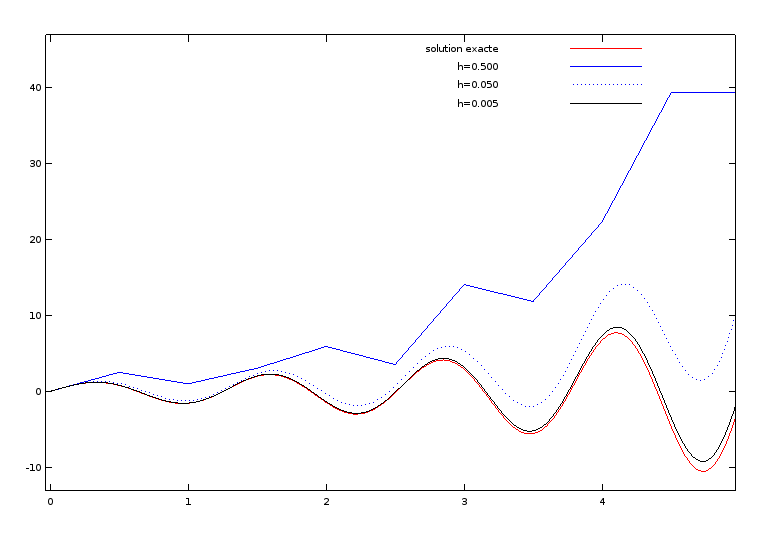
\includegraphics[scale=0.7]{./img/step-forward-euler.png}
    % step-forward-euler.png: 780x543 pixel, 96dpi, 20.63x14.37 cm, bb=0 0 585 407
\end{figure}

    Nous pouvons voir que pour $h = 0.5$ la méthode explode.

    Voir le fichier \emph{test\_methods.m} pour le code MATLAB.

    \item \emph{Tracer les courbes d’erreur de la méthode en échelle log-log et
    déterminer l'ordre de cette méthode: on tracera $\log(e(h)) = \log(\norm{y_h -
    y}{})$ en fonction de $\log(h)$ où $y_h$ désigne la solution approchée sur
    $[0, T]$ pour un certain pas $h$ et $y$ la solution exacte (ou du moins une
    solution très précise). On peut aussi utiliser l'erreur de consistance
    suivante (rappel: $h = \frac{1}{N}$):}
\[
    e(h) = \max_{0 \leq n \leq N} \abs{y_n - y(t_n)}{}.
\]

    Soit l'équation différentielle suivante:
\begin{equation}\label{eq:eq2}
\left\{
\begin{array}{ll}
    y'(t) = 2 - e^{-4t} - 2y(t) & \quad 0 \leq t \leq T \\
    y(0) = 1
\end{array}
\right.
\end{equation}

    Avec la solution exacte:
\[
    y(t) = 1 + \frac{1}{2} e^{-4t} - \frac{1}{2} e^{-2t}
\]
\clearpage
    L'ordre est:
\begin{figure}[h!]
    \centering
    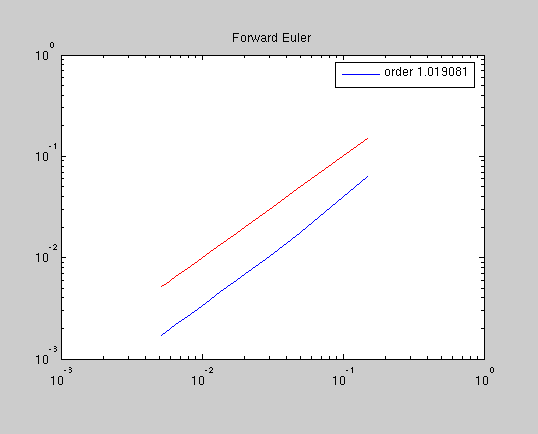
\includegraphics[scale=0.5]{./img/order-forward-euler.png}
    % order-forward-euler.png: 538x434 pixel, 72dpi, 18.98x15.31 cm, bb=0 0 538 434
\end{figure}

    Voir le fichier \emph{test\_methods\_order.m} pour le code MATLAB.
\end{enumerate}

\subsection{Euler Implicite}
La méthode d’Euler Implicite s’écrit:
\begin{equation}\label{eq:eulerim}
    y_{n + 1} = y_n + h f(t_{n + 1}, y_{n + 1}).
\end{equation}

\begin{enumerate}
    \item \emph{Remarquer que pour cette méthode il est nécessaire de résoudre un
    système à chaque étape. Remarquer de plus que si $f$ est non linéaire alors ce
    système devient nécessaire.}

    Notre inconnue, $y_{n + 1}$, est presente sur la gauche et sur la droite de
    l'équation. Si $f$ est une fonction linéaire on peut se ramener à une méthode
    explicite en deplaçant tous les termes contentant $y_{n + 1}$ vers la gauche,
    mais si $f$ est non-linéaire, cela est impossible et il faut que nous resolvons
    le système.

    \item \emph{Implémenter la méthode de Newton de recherche du zéro d’un système
    d’équation. La tester sur des cas simples de votre choix. Rappel: Pour trouver
    le zéro d'un fonction vectorielle $F: \field{R}^d \to \field{R}^d$ il faut
    résoudre itérativement le problème suivant:}
\begin{equation}\label{eq:newton}
    F'(s_n)(s_{n + 1} - s_n) = -F(s_n)
\end{equation}
avec $F'(s_n)$ la matrice jacobienne de $F$ en $s_n$.

    Voir le fichier \emph{NewtonSolver.m} pour le code MATLAB.

    \item \emph{Retrouver, par un raisonnement formel, pourquoi l'on doit résoudre le
    systéme \eqref{eq:newton}.}

    Soit $F: \field{R}^d \to \field{R}^d$ une fonction définie par:
\[
    F(y) = y - y_{n} - hf(t_{n + 1}, y)
\]
qui est obtenue à partir du système~\eqref{eq:eulerim}. Alors, la solution du système
\eqref{eq:newton} nous donne un zéro de $F$ qui est aussi une solution du
\eqref{eq:eulerim}.

    \item \emph{Implémenter la méthode d’Euler Implicite.}

    Voir le fichier \emph{BackwardEuler.m} pour le code MATLAB.

    \item \emph{Faire quelques cas tests sur des exemples simples. Se pose-t-il le
    même problème qu'avec Euler Explicite si le pas $h$ devient trop grand?}

     En utilisant le système~\eqref{eq:eq1}:
\begin{figure}[h!]
    \centering
    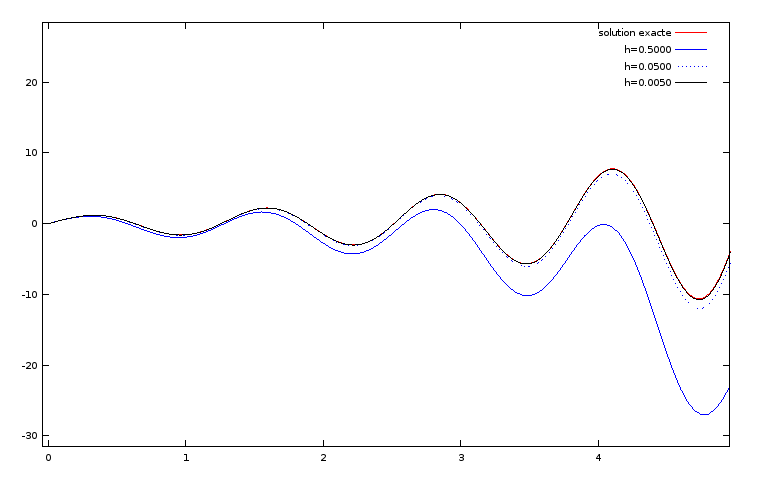
\includegraphics[scale=0.6]{./img/step-backward-euler.png}
\end{figure}

    Voir le fichier \emph{test\_methods.m} pour le code MATLAB.

    La méthode d'Euler Implicite est inconditionallement stable donc elle n'a pas
    des problèmes quand le pas devient trop grand.

    \item \emph{Tracer les courbes d'erreur de la méthode en échelle log-log et
    vérifier que l'ordre de cette méthode est le même que pour Euler Explicite.}

    En utilisant le système~\eqref{eq:eq2} on a l'ordre de la méthode:
\begin{figure}[h!]
    \centering
    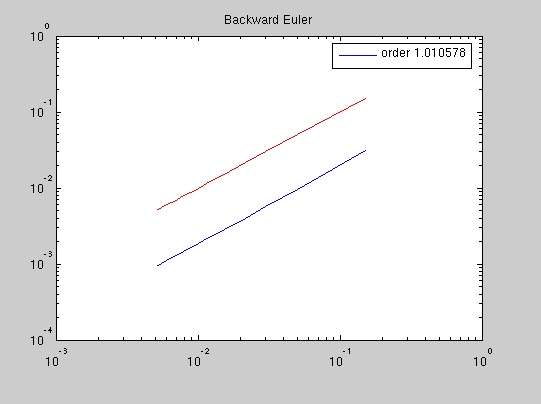
\includegraphics[scale=0.5]{./img/order-backward-euler.png}
    % order-backward-euler.png: 541x404 pixel, 72dpi, 19.09x14.25 cm, bb=0 0 541 404
\end{figure}

    Voir le fichier \emph{test\_methods\_order.m} pour le code MATLAB.
\end{enumerate}

\subsection{Problème raide}

Voici un exemple de problème raide (stiff problem). Considérons le problème de
Cauchy suivant:
\begin{equation}\label{eq:raide}
\left\{
\begin{array}{ll}
    y'(t) = -\lambda y + 1 + \lambda t, & \quad 0 \leq t \leq T \\
    y(0) = 1 &
\end{array}
\right.
\end{equation}

\begin{enumerate}
    \item \emph{Calculer la solution exacte.}

    La solution exacte est:
\[
    y(t) = e^{-\lambda t} + t
\]
    \item \emph{Prendre $\lambda = 600$. Comparer les méthodes d'Euler Explicite et
    Implicite lorsque $h = 0.01$ et $h = 0.001$.}

    Pour chaque méthode nous prenons:
\[
    e(h) = \max_{0 \leq n \leq N} \abs{y_n - y(t_n)}{}.
\]
avec les results suivantes:
\begin{center}
    \begin{tabular}{|l|l|l|}\hline
        h         & Euler Explicite         & Euler Implicite \\\hline
        $0.01$    & $1.2634e+30$            & $0.99617$ \\\hline
        $0.001$   & $0.99667$               & $0.99617$ \\\hline
    \end{tabular}
\end{center}

    \item \emph{En déduire un avantage de la méthode implicite sur la explicite. Ce
    problème est appelé ``raide'' car il nécessite un pas très petit pour
    converger avec du explicite.}

    Avec les resultats du question précédent nous pouvons conclure que la méthode
    implicite est meilleur que la méthode explicite parce qu'elle donne des resultats
    exactes pour tous valeur de $h$.

\end{enumerate}

\section{La méthode de Runge-Kutta 4}

La méthode de Runge-Kutta 4 s'écrit:
\begin{align}\nonumber
    k_1^n & = f(t_n, y_n) \\\nonumber
    k_2^n & = f(t_n + \frac{h}{2}, y_n + \frac{h}{2} k_1^n) \\
    k_3^n & = f(t_n + \frac{h}{2}, y_n + \frac{h}{2} k_2^n) \\\nonumber
    k_4^n & = f(t_{n + 1}, y_n + h k_3^n) \\\nonumber
    y_{n + 1} & = y_n + \frac{h}{6}(k_1^n + 2 k_2^n + 2k_3^n + k_4^n)
\end{align}

\begin{enumerate}
    \item \emph{Implémenter cette méthode.}

    Voir le fichier \emph{RungeKutta4.m} pour le code MATLAB.
\clearpage
    \item \emph{Faire quelques cas tests sur des exemples simples. Remarquer qu'il se
    pose des problèmes lorsque le pas $h$ devient trop grand.}

    En utilisant le système~\eqref{eq:eq1}:
\begin{figure}[h!]
    \centering
    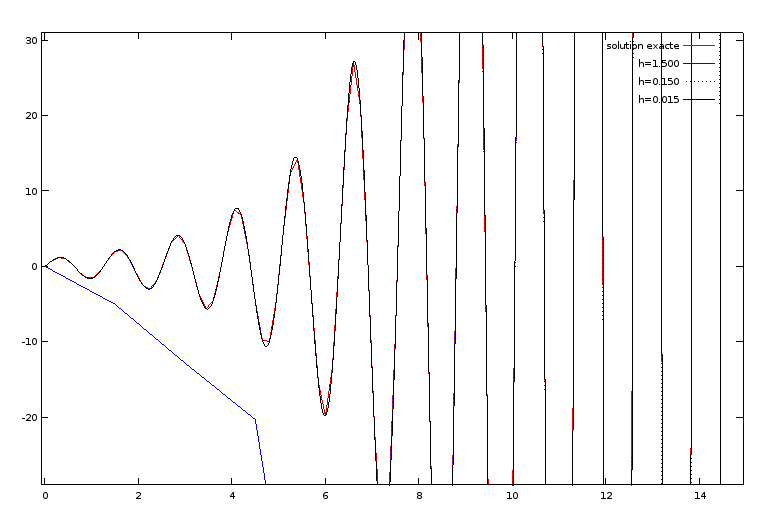
\includegraphics[scale=0.6]{./img/step-runge-kutta.png}
\end{figure}

    Voir le fichier \emph{test\_methods.m} pour le code MATLAB.

    \item \emph{Tracer les courbes d'erreur de la méthode en échelle log-log et
    déterminer l'ordre de cette méthode.}

    En utilisant le système~\eqref{eq:eq2} on a l'ordre de la méthode:
\begin{figure}[h!]
    \centering
    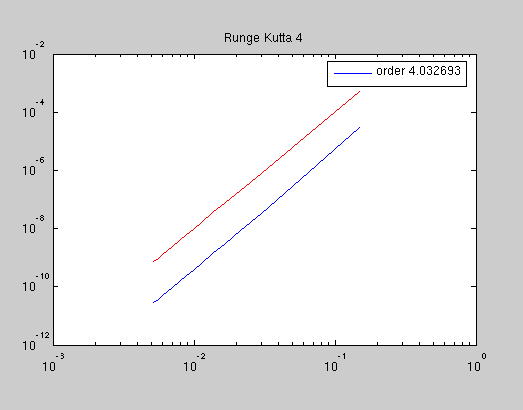
\includegraphics[scale=0.5]{./img/order-runge-kutta-4.png}
\end{figure}

    \item \emph{Résoudre le problème raide précédent en utilisant les mêmes données
    mais avec la méthode de RK4. Que remarque-t-on?}

\begin{center}
    \begin{tabular}{|l|l|}\hline
        h         & Runge-Kutta 4 \\\hline
        $0.01$    & $6.7650e+13$  \\\hline
        $0.001$   & $3.1743e-05$     \\\hline
    \end{tabular}
\end{center}

    On remarque que la méthode de Runge-Kutta 4 est une méthode explicite comme
    Euler Explicite et elle a les mêmes problèmes quand $h$ devient trop grand.
\end{enumerate}

\section{La méthode de Crank-Nicolson}

La méthode de Crank-Nicolson s'écrit:
\begin{align}
    y_{n + \frac{1}{2}} & = y_n + \frac{h}{2} f(t_n + \frac{h}{2}, y_{n + \frac{1}{2}})
    \\\nonumber
    y_{n + 1} & = y_n + hf(t_n + \frac{h}{2}, y_{n + \frac{1}{2}})
\end{align}

\begin{enumerate}
    \item \emph{Implémenter cette méthode. (méthode implicite donc utilisant la
    méthode de Newton précédemment implémentée).}

    Voir le fichier \emph{test\_methods.m} pour le code MATLAB.

    \item \emph{Faire quelques cas tests sur des exemples simples.}

    En utilisant le système~\eqref{eq:eq1}:
\begin{figure}[h!]
    \centering
    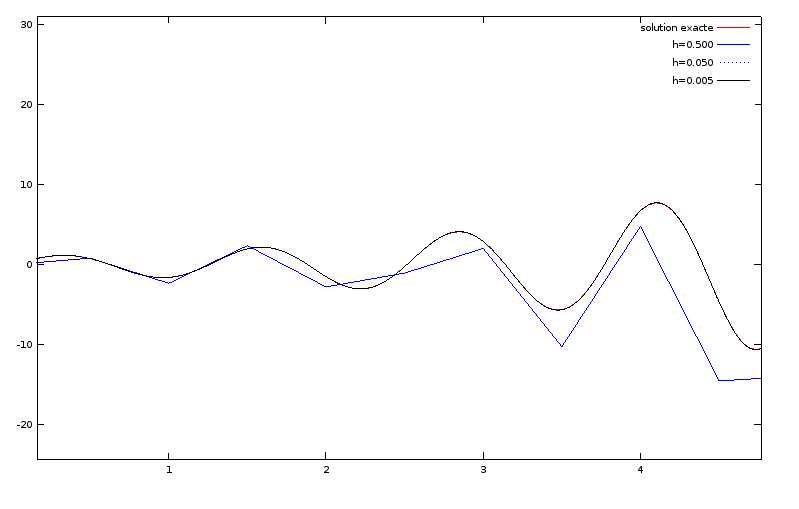
\includegraphics[scale=0.6]{./img/step-crank-nicolson.png}
\end{figure}

    Voir le fichier \emph{test\_methods.m} pour le code MATLAB.
\clearpage
    \item \emph{Tracer les courbes d'erreur de la méthode en échelle log-log et montrer
    que la méthode est d'ordre 2.}

    En utilisant le système~\eqref{eq:eq2} on a l'ordre de la méthode:
\begin{figure}[h!]
    \centering
    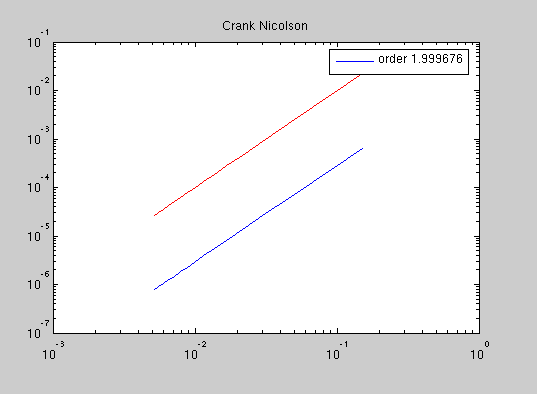
\includegraphics[scale=0.5]{./img/order-crank-nicolson.png}
\end{figure}

    \item \emph{Résoudre le problème raide précédent en utilisant les mêmes données mais
    avec la méthode de Crank-Nicolson. Que remarque-t-on?}

    \begin{center}
    \begin{tabular}{|l|l|}\hline
        h         & Crank-Nicolson \\\hline
        $0.01$    & $0.2497871$  \\\hline
        $0.001$   & $0.0027725$     \\\hline
    \end{tabular}
\end{center}

    On remarque que la méthode de Crank-Nicolson n'a pas des problèmes quand $h$
    devient trop grand car elle est une méthode implicite comme Euler Implicite.
\end{enumerate}

\section{Application au pendule pesant}
\emph{Considérons un pendule constitué d'une masse ponctuelle $m$ au bout d'une tige de
masse nulle et de tlongueur $L$, tournant sans frottement autour de l'axe orienté
dirigé par un vecteur horizontal $e$, et soumis à la pesanteur $g$ supposée uniforme.
On note $\theta$ l'angle que la tige fait avec la verticale et $\dot{\theta}$ la
vitesse angulaire de la tige.}

\begin{enumerate}
    \item \emph{Dessiner le problème (En LaTeX on pourra utiliser LaTeXDraw).}
\begin{figure}[h!]
    \centering
    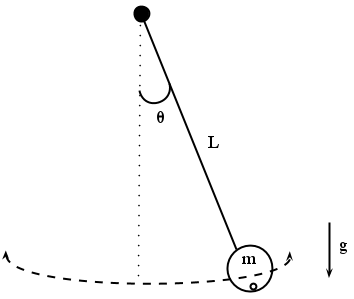
\includegraphics[scale=0.4]{./img/pendulum.png}
    % pendulum.png: 369x302 pixel, 72dpi, 13.02x10.65 cm, bb=0 0 369 302
\end{figure}

    \item \emph{Montrer que l'energie totale s'écrit :}
\[
    E_T = E_C + E_{PP} = \frac{1}{2} m L^2 \dot{\theta}^2 + m g L (1 - \cos(\theta))
\]

    \item \emph{Sachant que l'énergie totale se conserve, dériver l'expression pour
    obtenir l'équation de mouvement.}
\begin{align*}
    & \frac{\dx{}}{\dx{t}} (\frac{1}{2} m L^2 \dot{\theta}^2 + m g L (1 -
    \cos(\theta)) - E_T) = 0\\
    \equivto & m L^2 \ddot{\theta} + m g L \sin(\theta) = 0\\
    \equivto & \ddot{\theta} + \frac{g}{L} \sin(\theta) = 0
\end{align*}

    \item \emph{Décomposer cette équation différentielle du second ordre en un système
    d'équation différentielle du premier ordre. On notera $y_1 = \theta$,
    $y_2 = \dot{\theta}$ et $\omega_0 = \sqrt{\frac{g}{L}}$.}

    On peut se ramener à un système comme~\eqref{eq:eqdiff} où:
\[
    y(t) = \left(\!
    \begin{array}{c}
        y_1(t) \\
        y_2(t)
    \end{array}
  \!\right) \text{ et }
  y'(t) = f(t, y) = \left(\!
    \begin{array}{c}
        y_2(t)\\
        -\omega_0^2 \sin(y_1(t))
    \end{array}
  \!\right)
\]

    \item \emph{Résoudre le problème du pendule pesant sur un exemple de votre choix
    avec les conditions initiales de votre choix.}

    Voir le fichier \emph{test\_pendulum.m} pour le code MATLAB.

    \item \emph{Représenter l'évolution de la trajectoire dans l'espace des phases (i.e.
    tracer $y_2$ en fonction de $y_1$) lorsque la position initiale est
    $\frac{\pi}{2}$ et la vitesse initiale vaut $0.2$. Augmenter la vitesse initiale
    jusqu'à avoir un portrait de phase différent. Que veut dire ce nouveau portrait
    de phase par rapport au précédent?}

    Pour une vitesse initiale de $0.2$:
\begin{figure}[h!]
    \centering
    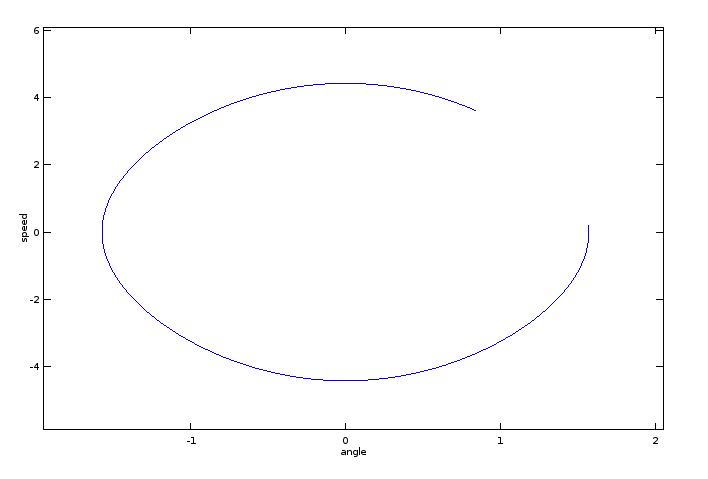
\includegraphics[scale=0.5]{./img/pendulum-phase1.png}
    % pendulum-phase1.png: 708x479 pixel, 96dpi, 18.73x12.67 cm, bb=0 0 531 359
\end{figure}
\clearpage
    Pour une vitesse initiale de $5$:
\begin{figure}[h!]
    \centering
    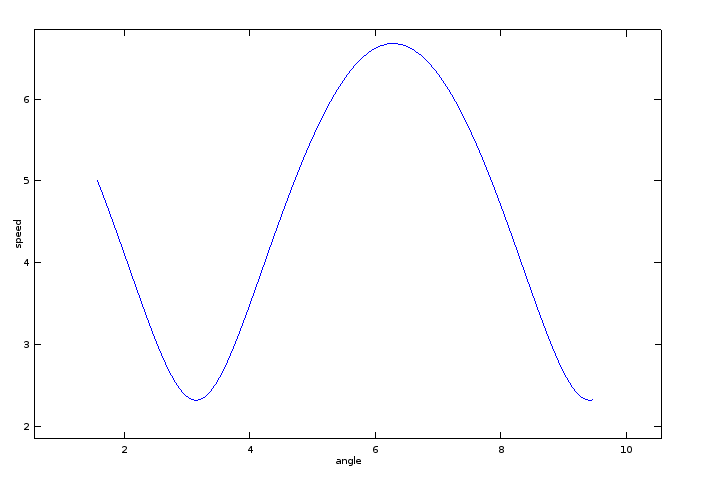
\includegraphics[scale=0.5]{./img/pendulum-phase.png}
    % pendulum-phase1.png: 708x479 pixel, 96dpi, 18.73x12.67 cm, bb=0 0 531 359
\end{figure}

    Dans la première figure, nous pouvons voir le pendule commençant sur ​​l'axe
    horizontal, à droite. En temps, il descend à être totalement verticale, avec une
    vitesse qui accroît. Après avoir passé la position verticale, il commence à
    perdre de la vitesse grace à la gravité et il tourne en arrière, avec une vitesse
    qui accroît encore. Il fait cela indéfiniment.

    Dans la deuxième figure, la vitesse initial est plus grande donc le pendule
    tourne indéfiniment autour de l'origine avec l'angle en constante augmentation.

    Voir le fichier \emph{test\_pendulum.m} pour le code MATLAB.

    \item \emph{Tracer l'évolution du portrait de phase lorsque la position initiale
    varie et la vitesse initiale est nulle. Dire quelles sont les positions
    ``stables'' (le pendule oscille indéfiniment sans faire le tour du point
    d'accrochage) et ``instables'' (le pendule tourne indéfiniment autour du point
    d’accrochage).}

\begin{figure}[ht]
    \begin{minipage}[b]{0.5\linewidth}
        \centering
        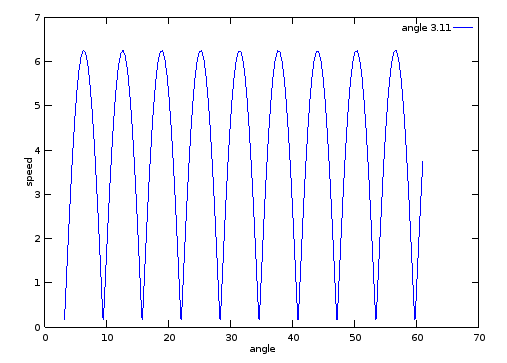
\includegraphics[scale=0.5]{./img/pendulum-unstable.png}
        \caption{Position instable}
    \end{minipage}
    \hspace{0.5cm}
    \begin{minipage}[b]{0.5\linewidth}
        \centering
        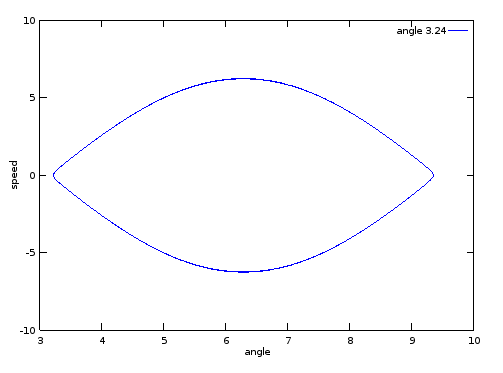
\includegraphics[scale=0.5]{./img/pendulum-stable.png}
        \caption{Position stable}
    \end{minipage}
\end{figure}

    Pour un vitesse initiale nulle tous les positions sont stables, mais avec un vitesse
    initiale $\dot{\theta}(0) = 0.2$ nous trouvons des positions instables aussi.
    Pour un angle compris entre $[3.08, 3.20]$ ($\approx \pi$, la position est presque
    vertical) nous avons des positions instables dans lesquelles le pendule tourne
    indéfiniment (l'angle augmente indéfiniment).

    Voir le fichier \emph{test\_pendulum.m} pour le code MATLAB.

    \item \emph{Regardons le cas où le pendule est amorti. L'équation s'écrit alors avec
    le coefficient d'amortissement $\alpha$:}
\[
    \ddot{\theta} = -\omega_0^2 \sin(\theta) - \alpha \dot{\theta}
\]

    Voir le fichier \emph{test\_pendulum.m} pour le code MATLAB.
\clearpage
    \item \emph{Tracer un portrait de phase en tenant compte de l'amortissement.
    Commenter.}
\begin{figure}[h!]
    \centering
    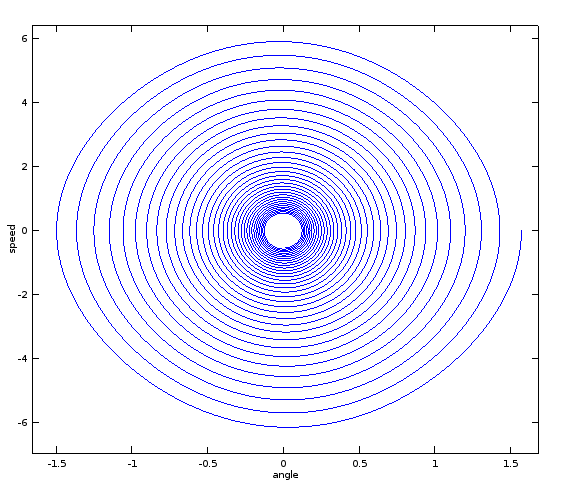
\includegraphics[scale=0.5]{./img/pendulum-friction.png}
    \caption{$\alpha = 0.1,~T = 50s,~\dot{\theta}(0) = 0,~\theta(0) = \frac{\pi}{2}$}
    % pendulum-friction.png: 607x504 pixel, 96dpi, 16.06x13.33 cm, bb=0 0 455 378
\end{figure}

    Avec l'amortissement nous pouvons voir que a chaque tour la vitesse du pendule
    diminue (elle tend vers 0).

    Voir le fichier \emph{test\_pendulum.m} pour le code MATLAB.
\end{enumerate}

\end{document}